\documentclass[conference]{IEEEtran}
\usepackage{graphicx}
\usepackage{hyperref}
\usepackage{cleveref}
\usepackage{url}
\usepackage{algorithm}
\usepackage{algpseudocode}
\usepackage{tikz}
\usepackage{booktabs}
\usetikzlibrary{arrows.meta, positioning, shapes.geometric, fit, backgrounds, calc}
\usepackage{listings}
\usepackage{xcolor}
\usepackage{multirow}
\usepackage{enumitem}
\usepackage{float}
\usepackage{amssymb}
\algnewcommand{\Try}{\textbf{try}}
\algnewcommand{\Catch}{\textbf{catch}}
\algnewcommand{\EndTry}{\textbf{end try}}
\lstset{
    basicstyle=\ttfamily\small,
    breaklines=true,
    frame=single,
    numbers=left,
    numberstyle=\tiny\color{gray},
    keywordstyle=\color{blue},
    commentstyle=\color{green!60!black},
    stringstyle=\color{red},
    showstringspaces=false,
    tabsize=4,
    captionpos=b
}

\title{AI-Powered Intelligent Document Verification and Automatic Stamping Robot System}

\author{
\IEEEauthorblockN{Yaokai Yang}
\IEEEauthorblockA{\textit{School of Advanced Technology} \\
\textit{Xi'an Jiaotong-Liverpool University} \\
Suzhou, China \\
yaokai.yang23@student.xjtlu.edu.cn}
\and
\IEEEauthorblockN{Xiang Lin}
\IEEEauthorblockA{\textit{School of Advanced Technology} \\
\textit{Xi'an Jiaotong-Liverpool University} \\
Suzhou, China \\
xiang.lin23@student.xjtlu.edu.cn}
\and
\IEEEauthorblockN{Xinyang Zhang}
\IEEEauthorblockA{\textit{School of Advanced Technology} \\
\textit{Xi'an Jiaotong-Liverpool University} \\
Suzhou, China \\
xinyang.zhang23@student.xjtlu.edu.cn}
\and
\IEEEauthorblockN{Yunxuan Wu}
\IEEEauthorblockA{\textit{School of Advanced Technology} \\
\textit{Xi'an Jiaotong-Liverpool University} \\
Suzhou, China \\
yunxuan.wu23@student.xjtlu.edu.cn}
\and
\IEEEauthorblockN{Haoran Zheng}
\IEEEauthorblockA{\textit{School of Advanced Technology} \\
\textit{Xi'an Jiaotong-Liverpool University} \\
Suzhou, China \\
haoran.zheng23@student.xjtlu.edu.cn}
}

\date{April 2026}

\begin{document}


\maketitle

\begin{abstract}
\textbf{Executive Summary:} This project presents an \textbf{AI-Powered Intelligent Document Verification and Automatic Stamping Robot System} designed for document approval automation in administrative offices, enterprises, educational institutions, and government service centers. The system employs a \textbf{three-tier architecture}---frontend interaction layer, backend management layer, and hardware execution layer---integrating optical character recognition (OCR), AI-driven intelligent document classification, RAG (Retrieval-Augmented Generation) based knowledge-enhanced verification, a multi-dimensional rule engine, and servo-controlled physical stamping into a unified intelligent automation pipeline. The system implements a complete closed-loop workflow: \textbf{input $\rightarrow$ recognition $\rightarrow$ reasoning $\rightarrow$ decision $\rightarrow$ execution $\rightarrow$ logging $\rightarrow$ analytics}. The backend management layer provides a visual analytics dashboard covering approval pass rates, document type distribution, processing trend analysis, and anomaly monitoring. All operations generate comprehensive audit logs with before-and-after stamping image comparisons, ensuring full traceability. Documents with ambiguous validation results are automatically routed to a human review queue, enabling \textbf{human-AI collaborative} approval. The total hardware cost is approximately \textyen\,240, making it a low-cost, efficient, and scalable administrative automation solution.
\end{abstract}

%=============================================================================
\section{Background and Motivation}
%=============================================================================

\subsection{Industry Background and Problem Statement}

In administrative offices, enterprise approval workflows, educational institutions, and government service centers, document processing---including leave applications, expense reimbursements, certificate issuance, and contract signing---has long relied on manual review and physical stamping. Statistics indicate that administrative personnel spend over 30\% of their working hours on repetitive paperwork. This workflow faces the following critical challenges:

\begin{itemize}[leftmargin=*]
    \item \textbf{Efficiency Bottleneck:} Staff must manually read each document, verify fields against databases, and physically apply stamps, processing only 10--15 documents per hour, leading to backlogs during peak periods.
    \item \textbf{Human Error Risk:} Manual verification is prone to overlooking missing fields, expired dates, or mismatched identity information, with error rates increasing under workload fatigue.
    \item \textbf{Compliance and Audit Gaps:} The lack of systematic audit trails makes it difficult to trace approval timelines, accountability, and operation records, creating governance blind spots.
    \item \textbf{Stamp Security Vulnerabilities:} Physical stamps are frequently left unsecured, risking unauthorized use, duplication, or tampering.
    \item \textbf{Low Data Utilization:} Vast amounts of approval data exist only in paper form, failing to generate analyzable and optimizable operational insights.
\end{itemize}

\subsection{Motivation and Technical Opportunities}

With the maturation of AI vision technologies (such as PaddleOCR for Chinese-optimized OCR engines), the proliferation of low-cost microcontrollers (Arduino), and the exploration of Retrieval-Augmented Generation (RAG) in document understanding, building an \textbf{intelligent, low-cost, reproducible} document approval automation system has become feasible. This project aims to:

\begin{enumerate}[leftmargin=*]
    \item Replace manual document review with \textbf{AI-driven intelligent document recognition}, enabling automatic document type classification and content understanding.
    \item Introduce \textbf{RAG knowledge-enhanced verification} to cross-reference OCR results with institutional policies and historical approval records, reducing recognition hallucinations and misjudgments.
    \item Achieve \textbf{physical stamping automation} through servo-controlled force regulation and an anti-tamper locking mechanism, ensuring stamping quality and security.
    \item Build a backend management platform with \textbf{visual analytics and operational insights}, transforming approval data into quantifiable operational intelligence.
    \item Provide a \textbf{role-based Web interface} enabling separation of duties and human-AI collaborative approval among operators, reviewers, and administrators.
\end{enumerate}

\subsection{Project Scope}

This project is developed as part of \textbf{MEC202 -- Specific General Project 9} at Xi'an Jiaotong-Liverpool University, under the supervision of Dr.\ Bangxiang Chen. The system targets four typical document types (leave applications, expense reimbursements, certificates, and general documents) using a university administrative setting as the validation environment. The system design fully considers \textbf{extensibility}, supporting flexible adaptation to different institutional document types and approval rules through a template management mechanism.

%=============================================================================
\section{System Design and Technical Approach}
%=============================================================================

\subsection{System Architecture}

The system employs a \textbf{three-tier architecture} as illustrated in \Cref{fig:architecture}. This architecture divides the system into three collaborative layers, achieving a complete closed loop from user interaction to physical execution:

\begin{figure}[H]
\centering
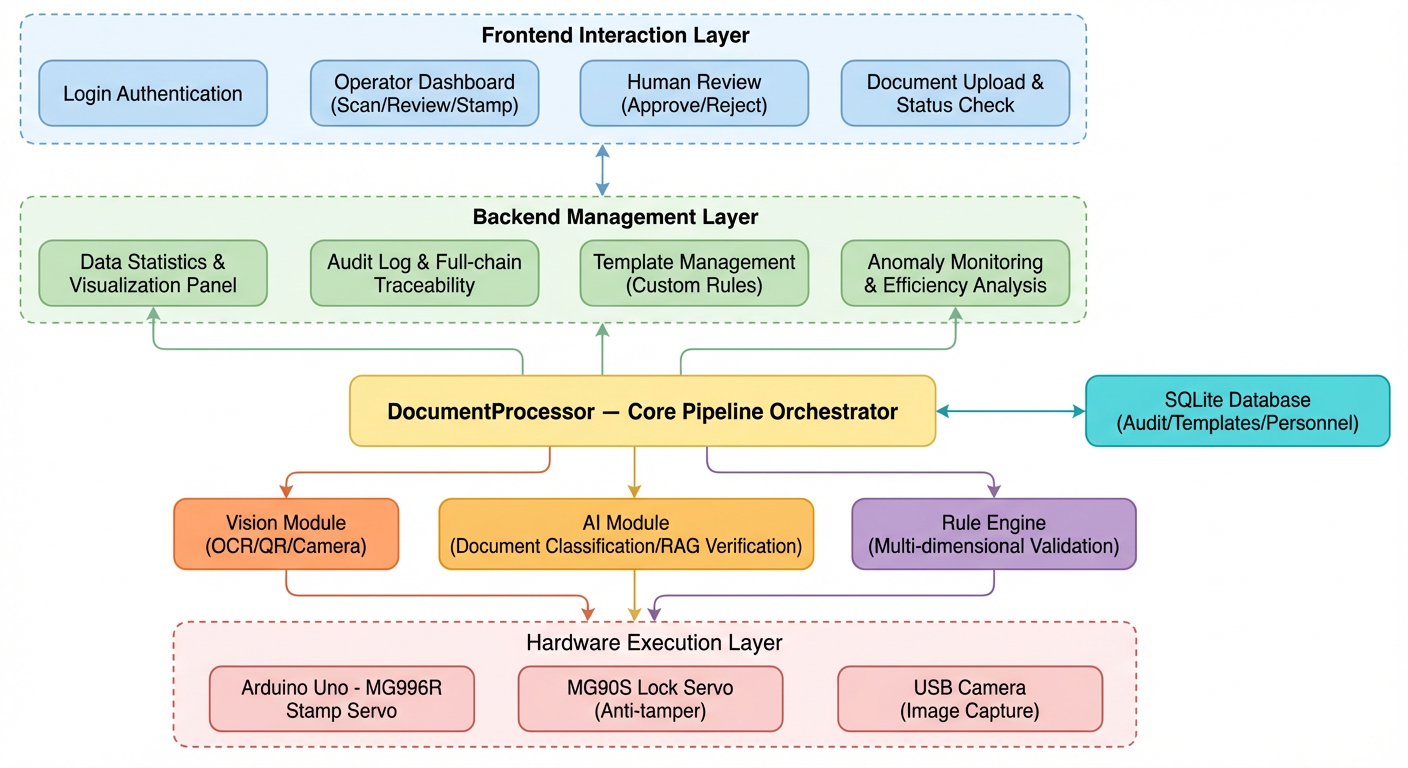
\includegraphics[width=0.5\textwidth]{845afd78c54c4bc0e2f78b941e47ca60.png}
\caption{System three-tier architecture overview: frontend interaction layer, backend management layer, and hardware execution layer working collaboratively, orchestrated by the core pipeline controller.}
\label{fig:architecture}
\end{figure}

\textbf{Layer 1---Frontend Interaction Layer:} A Flask-based Web application serving three user roles: operators, reviewers, and administrators. It provides task submission, document scanning and review, human review processing, and status query functions. Role-based access control (RBAC) ensures that users can only access functions corresponding to their permission level.

\textbf{Layer 2---Backend Management Layer:} Provides institutional operations management capabilities, including:
\begin{itemize}[leftmargin=*]
    \item \textbf{Visual Analytics Dashboard:} Real-time display of approval pass rates, document type distribution, processing trends, and anomaly ratios, assisting management in workflow optimization and resource allocation.
    \item \textbf{Full-chain Audit Logs:} Every document processing event records complete metadata (operator, timestamp, OCR results, validation details, before-and-after stamping images), supporting multi-dimensional search by time, type, and operator.
    \item \textbf{Document Template Management System:} Administrators can create, edit, and delete document type templates through a visual interface, defining required fields, optional fields, forbidden fields, and custom validation rules for each document type, extending supported document types without code modification.
    \item \textbf{Anomaly Monitoring and Efficiency Analysis:} Automatic identification of high-frequency rejection reasons, processing bottlenecks, and anomaly patterns, providing data-driven support for workflow improvement.
\end{itemize}

\textbf{Layer 3---Hardware Execution Layer:} An Arduino Uno microcontroller coordinates the USB camera, stamping servo, and locking servo to perform image capture and physical stamping operations. It communicates with the upper software layer via serial communication (9600 baud rate).

\subsection{Complete Processing Pipeline}

The system implements a complete automated pipeline from document input to stamped delivery, with the core workflow consisting of 10 stages as shown in \Cref{fig:flowchart}. This pipeline embodies the seven-step closed-loop design philosophy: \textbf{input $\rightarrow$ recognition $\rightarrow$ reasoning $\rightarrow$ decision $\rightarrow$ execution $\rightarrow$ logging $\rightarrow$ analytics}.

\begin{figure}[H]
\centering
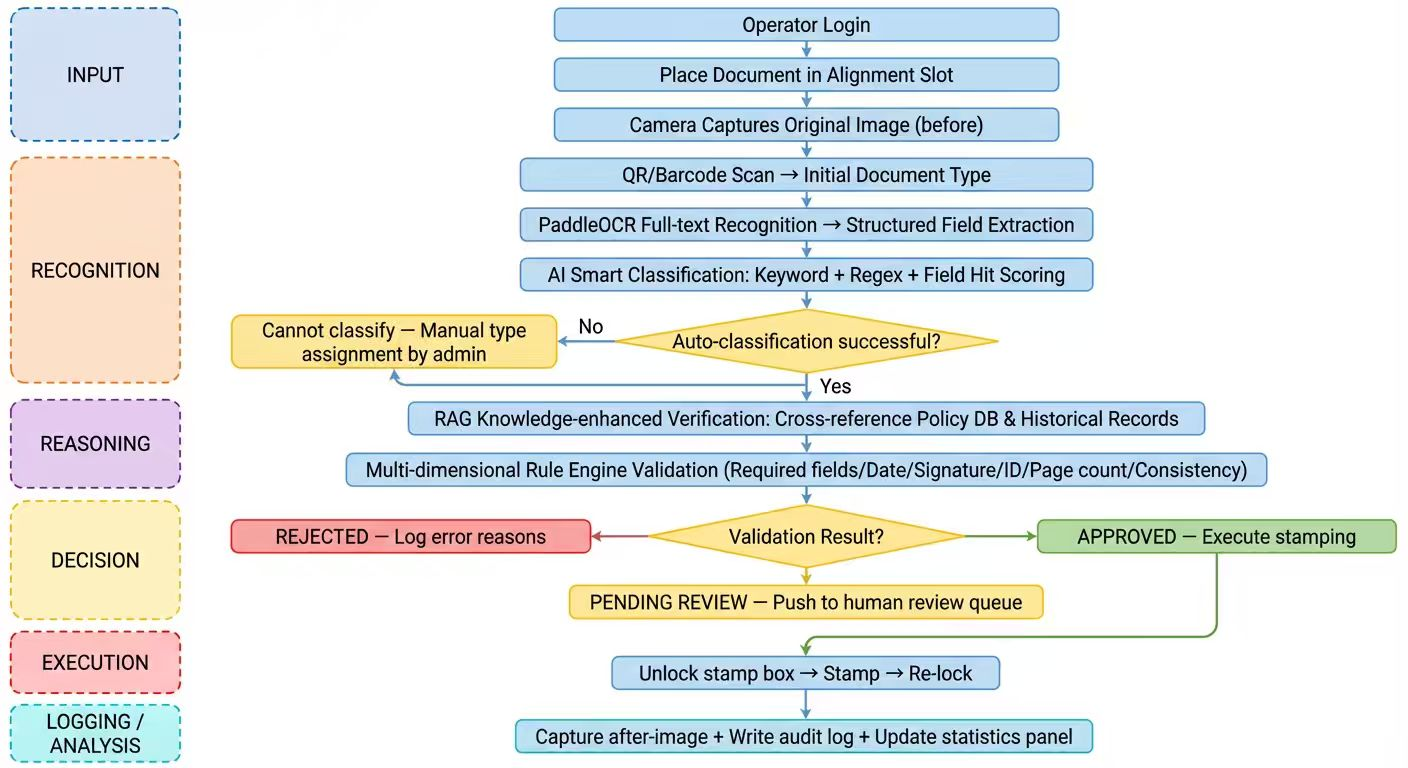
\includegraphics[width=0.5\textwidth]{54b1033c17ddb3bd7cd65716eb862d0e.jpg}
\caption{Intelligent document processing pipeline: seven-step closed loop (input $\rightarrow$ recognition $\rightarrow$ reasoning $\rightarrow$ decision $\rightarrow$ execution $\rightarrow$ logging $\rightarrow$ analytics), with three decision outcomes---rejection, human review, and approval with stamping.}
\label{fig:flowchart}
\end{figure}

\subsection{Key Technical Components}

\subsubsection{Vision Module}

The vision module (\texttt{vision/}) handles all image acquisition and text recognition, serving as the system's ``perception'' entry point:

\begin{itemize}[leftmargin=*]
    \item \textbf{Camera Control} (\texttt{camera.py}): Manages the USB camera via OpenCV, with automatic warm-up (discarding the first 3 frames to stabilize exposure) and timestamped file naming, ensuring consistency and traceability of image acquisition.
    \item \textbf{OCR Engine} (\texttt{ocr.py}): Employs PaddleOCR with Chinese-English mixed recognition and angle classification support. Regex patterns optimized for Chinese university forms convert unstructured text into structured fields (name, student ID, date, amount, reason, etc.), providing a data foundation for subsequent validation.
    \item \textbf{QR Code Scanning} (\texttt{qr\_scanner.py}): Decodes QR codes and barcodes via pyzbar + OpenCV for rapid initial document type identification, reducing the computational overhead of AI classification.
    \item \textbf{AI Document Intelligent Classification} (\texttt{classifier.py}): When QR codes do not provide a clear document type, the system automatically activates the AI classification engine. This engine employs a multi-feature fusion scoring strategy---\textbf{keyword semantic matching} (weight 0.5), \textbf{regex pattern recognition} (weight 0.3), and \textbf{required field hit rate} (weight 0.5)---to comprehensively score candidate document types. When the gap between the highest and second-highest scores is below the threshold (0.05), the system identifies the document as ambiguous and automatically routes it to human review, preventing misclassification.
\end{itemize}

\subsubsection{RAG Knowledge-Enhanced Verification Module}

To reduce OCR recognition hallucinations and the limitations of rule-based engines, the system introduces the design philosophy of \textbf{Retrieval-Augmented Generation (RAG)}, constructing a knowledge-assisted verification mechanism:

\begin{itemize}[leftmargin=*]
    \item \textbf{Institutional Policy Knowledge Base:} Approval policies, validity period regulations, and field requirements for each document type are structured into a local knowledge base. OCR extraction results are cross-referenced with the knowledge base to verify whether field values comply with currently effective policy requirements.
    \item \textbf{Historical Approval Record Retrieval:} The system retrieves historical approval results for similar documents, assisting in determining whether the current document belongs to common anomaly patterns (e.g., frequently occurring field error types), improving anomaly detection accuracy.
    \item \textbf{Hallucination Suppression Mechanism:} When OCR extraction results conflict with known constraints in the knowledge base (e.g., the extracted date format does not conform to any known date specification), the system flags it as ``low recognition confidence'' and triggers human review rather than blindly trusting the OCR output.
\end{itemize}

\noindent This design upgrades pure rule-based validation to \textbf{knowledge-driven intelligent verification}, effectively reducing the risk of incorrect stamping caused by OCR misrecognition.

\subsubsection{Multi-Dimensional Rule Engine}

The validation module (\texttt{validator/}) implements a dynamic rule engine based on the template database, supporting administrator-configurable validation rules through the Web interface without code modification:

\begin{table}[H]
\centering
\caption{Multi-dimensional validation rule system with error classification.}
\label{tab:validation}
\begin{tabular}{@{}llp{4.5cm}@{}}
\toprule
\textbf{Validation Dimension} & \textbf{Method} & \textbf{Description} \\
\midrule
Required Field Completeness & Dynamic check per document template & Configurable via template management UI \\
Date Legality & Format + future date + staleness check & $>$90 days triggers soft warning \\
Signature/Approval Detection & OCR text keyword search & Detects signature/approval keywords \\
ID Cross-verification & SQLite personnel database query & Student ID and name matching \\
Document Type Consistency & QR code vs.\ AI classification comparison & Multi-source verification \\
Page Completeness & ``Page X of Y'' regex matching & Prevents missing page submission \\
Forbidden Field Detection & Template-defined forbidden field list & Detects fields that should not appear \\
Custom Field Rules & Regex/range/enum/length & Administrator-configurable flexible rules \\
\bottomrule
\end{tabular}
\end{table}

\noindent Validation results are classified into two levels: \textbf{hard errors} cause immediate rejection; \textbf{soft warnings} route documents to the human review queue, where reviewers make the final decision, enabling human-AI collaborative approval.

\subsubsection{Hardware Execution Module}

The hardware module (\texttt{hardware/stamp.py}) communicates with an Arduino Uno via serial port (9600 baud rate) to achieve precise physical stamping control:

\begin{enumerate}[leftmargin=*]
    \item \textbf{Unlock} the stamp box (MG90S servo rotates to release the latch).
    \item \textbf{Stepped press-down}: The MG996R servo moves in 3\textdegree{} steps at 25\,ms intervals for controlled-force uniform stamping.
    \item \textbf{Hold} for 900\,ms to ensure clear ink transfer.
    \item \textbf{Slow release} and \textbf{re-lock} the stamp box to prevent unauthorized use.
\end{enumerate}

\noindent The Arduino firmware (\texttt{stamp\_controller.ino}) accepts four serial commands: \texttt{S} (stamp), \texttt{L} (lock), \texttt{U} (unlock), \texttt{P} (heartbeat/ping), ensuring reliable hardware-software communication.

\subsubsection{Data Analytics and Visualization}

The backend management platform features a Chart.js-based analytics dashboard providing visual analysis of the following core operational metrics:

\begin{itemize}[leftmargin=*]
    \item \textbf{Summary Metric Cards}: Total processing volume, approved count and pass rate, rejected count and rejection rate, pending review queue length---providing at-a-glance system status.
    \item \textbf{Document Type Distribution}: Doughnut chart showing submission proportions of each document type (leave/expense/certificate/general), helping management understand business composition.
    \item \textbf{Approval Result Distribution}: Doughnut chart displaying the ratio of approved/rejected/pending review, visually reflecting approval quality.
    \item \textbf{Processing Trend Analysis}: Line chart supporting 7-day and 30-day dimensions, showing daily approval volume changes for identifying business peaks and troughs.
    \item \textbf{Recent Processing Records}: Real-time updated processing log table, including timestamp, operator, document type, and approval result.
\end{itemize}

\noindent This analytics panel transforms the traditional ``black-box stamping'' into a \textbf{data-driven operations management tool}, enabling management to optimize approval workflows, allocate human resources rationally, and continuously monitor system efficiency and anomaly patterns based on objective data.

\subsubsection{Exception Handling and Fault Tolerance}

As a system involving hardware-software coordination for real-world deployment, robust exception handling is critical for reliable operation. The system implements comprehensive fault tolerance and degradation mechanisms across three dimensions---\textbf{hardware layer, document recognition layer, and software system layer}---following the design principles of \textbf{safety first, graceful degradation, and human fallback}.

\paragraph{Hardware Exception Handling}

Hardware-layer exceptions may cause physical operation failures or safety hazards. The system employs multiple protection measures:

\begin{itemize}[leftmargin=*]
    \item \textbf{Arduino Connection Failure:} The system proactively detects the serial connection on startup. Upon failure, it raises an exception containing diagnostic information (port name, troubleshooting steps), guiding the operator to quickly identify the issue (loose USB cable, incorrect port configuration, firmware not uploaded, etc.).
    \item \textbf{Stamping Process Exception:} The stamping sequence employs an \textbf{exception-safe} design---the \texttt{stamp()} method executes the stamping operation within a \texttt{try-catch} block, and \textbf{regardless of success or failure, forcibly executes stamp box locking under \texttt{finally} semantics}, preventing the stamp box from remaining in an unlocked state due to an interruption and eliminating safety hazards.
    \item \textbf{Arduino Heartbeat Detection:} The system periodically checks Arduino online status via the \texttt{P} command, expecting a \texttt{PONG} response to confirm normal communication. Heartbeat failure triggers a warning log, prompting the operator to check the hardware connection.
    \item \textbf{Camera Failure:} The initialization phase detects whether the camera opens normally (\texttt{isOpened()}), and the capture phase catches read failure exceptions and raises clear error messages, preventing empty-frame images from producing invalid OCR results downstream.
\end{itemize}

\paragraph{Document Content and Format Exceptions}

The diversity and non-standardization of document content are the primary challenges encountered in real-world deployment. The system addresses these through multi-level strategies:

\begin{itemize}[leftmargin=*]
    \item \textbf{Missing QR/Barcode:} When a document has no QR code or scanning fails, the system does not directly reject it but instead \textbf{automatically degrades to the AI intelligent classification engine} (\texttt{classifier.py}), determining the document type through multi-feature fusion scoring to ensure workflow continuity.
    \item \textbf{AI Classification Ambiguity:} When scores for multiple document types are too close (gap $<$ 0.05), the system identifies the document as \textbf{ambiguous}, avoids risky automatic classification, and routes it to the human review queue for manual type assignment by an administrator, preventing misclassification.
    \item \textbf{Incomplete OCR Field Extraction:} The OCR engine may miss fields due to image quality or font variations. The system automatically detects missing items through \textbf{required field completeness validation}, generating specific error messages (e.g., ``Missing required field: Student ID'') rather than producing ambiguous failures.
    \item \textbf{Date Format Diversity:} The system supports regex matching for multiple common Chinese date formats (\texttt{YYYY-MM-DD}, \texttt{YYYY/MM/DD}), and performs targeted detection of anomalous dates (future dates, excessively early years), classifying them as hard errors or soft warnings respectively.
    \item \textbf{Student ID Fallback Recognition:} When the standard format (with ``Student ID'' prefix) is not matched, the OCR module \textbf{automatically degrades to a continuous digit matching mode} (8--12 digits), improving recognition fault tolerance.
    \item \textbf{Multi-page Document Incompleteness:} Verifies multi-page document completeness by detecting ``Page X of Y'' format via OCR, preventing documents with missing pages from passing approval.
\end{itemize}

\paragraph{Software System Exceptions}

\begin{itemize}[leftmargin=*]
    \item \textbf{External System Integration Degradation:} When DMS (Document Management System) upload fails, the system only logs a warning and \textbf{does not affect the local approval and stamping workflow}, ensuring core functionality is not interrupted by external system unavailability. Personnel information queries similarly fall back to the local database upon DMS query failure.
    \item \textbf{Template Database Loading Failure:} The rule engine attempts to load document template definitions from the database; upon failure, it \textbf{automatically falls back to static rules in the configuration file} (\texttt{config.py}), ensuring validation functionality remains available at all times.
    \item \textbf{Regex/JSON Parsing Exceptions:} Custom validation rules may contain syntax errors in regex expressions or JSON configurations. The system catches \texttt{re.error} and \texttt{JSONDecodeError}, skipping individual erroneous rules rather than crashing the entire validation pipeline.
    \item \textbf{Web API Layer Exceptions:} Flask routes provide unified exception handling that returns structured JSON error responses (with error descriptions and HTTP status codes), enabling the frontend to display user-friendly error messages.
    \item \textbf{Simulation Mode:} The system includes a built-in \textbf{SIMULATION\_MODE} configuration switch that automatically skips all serial communication in hardware-less environments, replacing physical operations with log output, supporting development debugging and pure software demonstration.
\end{itemize}

\noindent The design principles of the exception handling mechanisms can be summarized as: \textbf{safety operations must have fallbacks} (forced locking on stamping exception), \textbf{non-core features can degrade} (DMS, external queries), \textbf{uncertain results go to humans} (ambiguous classification, soft warnings), and \textbf{all exceptions leave traces} (written to audit logs), ensuring the system operates safely and controllably under all exception scenarios.

\subsection{Physical Structure Design}

The device frame employs a \textbf{cost-oriented prototype validation approach}, using KT foam board (A3, 5\,mm thickness) for the main structure. This design choice is based on the following considerations:

\begin{itemize}[leftmargin=*]
    \item \textbf{Rapid Iteration:} KT board is easy to cut and modify, suitable for quickly adjusting layouts and testing different design approaches during the prototyping phase.
    \item \textbf{Cost Control:} Frame material costs only \textyen\,15, validating the system's feasibility at minimal cost, reflecting the project's focus on \textbf{cost-effectiveness}.
    \item \textbf{Portability:} Once prototype validation is complete, the main structure can be directly migrated to acrylic, aluminum alloy, or sheet metal for production, with no changes required to the hardware-software interfaces.
    \item \textbf{Avoiding 3D Printing Dependence:} Compared to 3D printing solutions (high per-unit cost, long print time, unsuitable for mass production), the KT board approach better aligns with cost control and production-oriented design thinking.
\end{itemize}

\noindent The design includes: \textbf{L-shaped alignment guides} ensuring consistent paper positioning; a \textbf{top crossbeam} mounting the camera for overhead document capture; \textbf{side-mounted servo arms} with the stamp attached to the servo horn endpoint; and an \textbf{anti-tamper locking mechanism} using a secondary servo controlling a physical latch.

\begin{figure}[H]
\centering
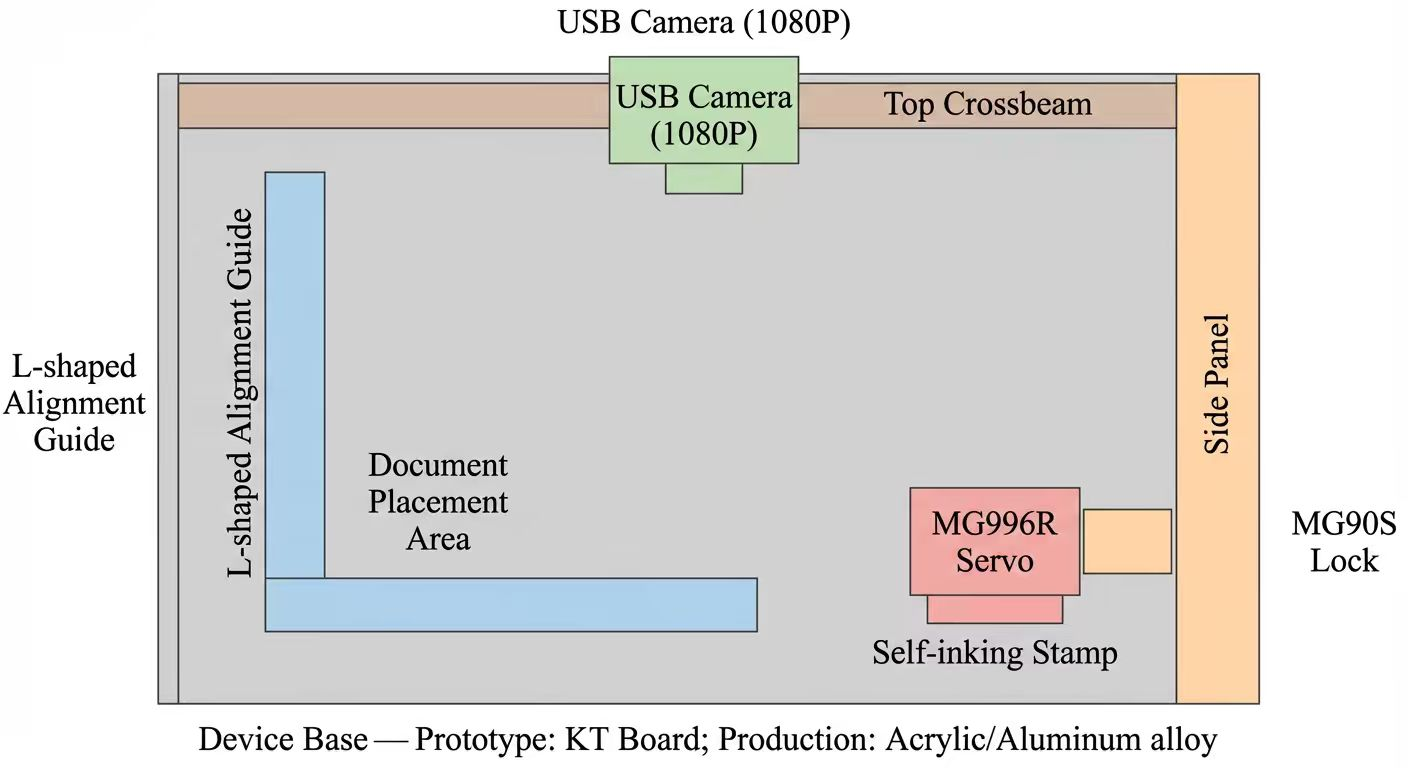
\includegraphics[width=0.5\textwidth]{1909a9044cfacd0bbe122ac6ad0ba1b4.jpg}
\caption{Top-down schematic of the physical device frame showing component placement. Prototype phase uses KT board; production phase can migrate to industrial materials.}
\label{fig:physical}
\end{figure}

%=============================================================================
\section{Deliverables and Goals}
%=============================================================================

\subsection{Primary Deliverables}

\begin{table}[H]
\centering
\caption{Project deliverables with acceptance criteria.}
\label{tab:deliverables}
\begin{tabular}{@{}p{4.5cm}p{5cm}c@{}}
\toprule
\textbf{Deliverable} & \textbf{Acceptance Criteria} & \textbf{Status} \\
\midrule
AI Document Classification & Multi-feature fusion scoring, ambiguity auto-flagging & \checkmark \\
OCR Structured Field Extraction & $\geq$90\% accuracy on real university forms & \checkmark \\
RAG Knowledge-Enhanced Verification & Cross-reference policy DB, suppress OCR hallucination & \checkmark \\
Multi-Dimensional Rule Engine & Covers all doc types, supports custom rules & \checkmark \\
Automatic Stamping Execution & Servo step control, adjustable force, anti-tamper lock & \checkmark \\
Human-AI Collaborative Review Queue & Web-based approve/reject workflow & \checkmark \\
Visual Analytics Dashboard & Pass rate/type distribution/trend analysis & \checkmark \\
Full-chain Audit Logs & Before/after images + full metadata + multi-dim search & \checkmark \\
Document Template Management & Visual create/edit templates, zero-code extension & \checkmark \\
Role-based Access Control & operator / reviewer / admin roles & \checkmark \\
DMS System Integration & REST API client & \checkmark \\
Simulation Mode & Full demo without hardware & \checkmark \\
\bottomrule
\end{tabular}
\end{table}

\subsection{Development Timeline}

\begin{table}[H]
\centering
\caption{Six-week development timeline.}
\label{tab:timeline}
\begin{tabular}{@{}clp{7cm}@{}}
\toprule
\textbf{Week} & \textbf{Focus Area} & \textbf{Key Activities} \\
\midrule
1 & Hardware Setup \& Base Architecture & Procure components, build frame, wire Arduino, upload firmware, set up Flask base framework \\
2 & AI Recognition \& Rule Engine & PaddleOCR integration and tuning, AI document classifier development, complete multi-dimensional validation rules \\
3 & Web Application \& Backend Management & Build frontend pages (login/dashboard/review), develop analytics dashboard and template management system \\
4 & System Integration \& RAG Verification & Connect all modules via \texttt{main.py}, implement RAG knowledge retrieval and hallucination suppression \\
5 & Testing, Tuning \& Analytics & End-to-end testing, optimize OCR regex and servo parameters, refine statistics and anomaly analysis \\
6 & Documentation \& Presentation & Record demo video, write project report, prepare presentation \\
\bottomrule
\end{tabular}
\end{table}

\subsection{Team Division}

\begin{table}[H]
\centering
\caption{Team member responsibilities and core deliverables.}
\label{tab:team}
\begin{tabular}{@{}llp{3cm}p{4cm}@{}}
\toprule
\textbf{Member} & \textbf{Role} & \textbf{Core Files} & \textbf{Deliverable} \\
\midrule
A (Hardware) & Frame + Arduino & \texttt{stamp\_controller.ino}, \texttt{hardware/} & Accurate stamping, alignment, lock mechanism \\
B (Vision) & OCR + AI Classification + Camera & \texttt{vision/} & $\geq$90\% field extraction, accurate AI classification \\
C (Logic) & Rule Engine + RAG Verification & \texttt{validator/}, RAG module & All doc type rules covered, effective hallucination suppression \\
D (Frontend) & Web Interface + Analytics Dashboard & \texttt{web/}, \texttt{templates/} & All pages functional, complete visualization dashboard \\
E (Integration) & Database + Pipeline + Templates & \texttt{main.py}, \texttt{database/} & End-to-end pipeline working, template management operational \\
\bottomrule
\end{tabular}
\end{table}

%=============================================================================
\section{Required Resources and Budget}
%=============================================================================

\subsection{Hardware Budget}

\begin{table}[H]
\centering
\caption{Hardware procurement list with estimated costs.}
\label{tab:budget}
\begin{tabular}{@{}cllc@{}}
\toprule
\textbf{\#} & \textbf{Component} & \textbf{Specification} & \textbf{Cost (\textyen)} \\
\midrule
1 & Arduino Uno R3 & Compatible + USB cable & 40 \\
2 & MG996R Servo & Metal gear, 10\,kg$\cdot$cm torque & 25 \\
3 & MG90S Servo & Micro servo for lock mechanism & 15 \\
4 & USB Webcam & 1080P, wide-angle, driver-free & 60 \\
5 & Self-inking Stamp & Custom ``Verified'' text, 4\,cm diameter & 25 \\
6 & KT Foam Board & A3 white, 5\,mm, 3 sheets & 15 \\
7 & Hot Glue Gun Set & With glue sticks & 20 \\
8 & Dupont Wires & Male-to-female, 20\,cm, 40-pack & 8 \\
9 & Acrylic Box & Small, for stamp storage & 15 \\
\midrule
 & & \textbf{Total} & \textbf{\textyen\,223} \\
\bottomrule
\end{tabular}
\end{table}

\subsection{Software Stack}

All software used is open-source and free of charge:

\begin{itemize}[leftmargin=*]
    \item \textbf{Python 3.10+} --- Main programming language
    \item \textbf{PaddleOCR 2.7.3} + \textbf{PaddlePaddle 2.6.1} --- Chinese-optimized OCR engine
    \item \textbf{Flask 3.0.3} --- Web framework
    \item \textbf{OpenCV 4.9} --- Image processing
    \item \textbf{Chart.js 4.4} --- Frontend data visualization
    \item \textbf{SQLite 3} --- Embedded database (no server needed)
    \item \textbf{Arduino IDE} --- Firmware development
\end{itemize}

\subsection{Development Environment}

\begin{itemize}[leftmargin=*]
    \item Operating System: Windows / macOS / Linux
    \item Memory: 4\,GB+ (PaddleOCR model requires $\sim$1.5\,GB RAM)
    \item Disk Space: $\sim$500\,MB for models and dependencies
    \item Network: Required for initial PaddleOCR model download ($\sim$300\,MB)
\end{itemize}

\subsection{Budget Summary}

With a total project budget of \textyen\,1,500, the hardware expenditure of \textyen\,223 leaves \textbf{\textyen\,1,277} for contingency, replacement parts, frame material upgrades (e.g., migrating from KT board to acrylic or aluminum alloy), or feature extensions.

%=============================================================================
\section*{Contribution Form}
%=============================================================================

\begin{table}[H]
    \centering
    \caption{Individual contribution breakdown.}
    \label{tab:contribution}
    \begin{tabular}{|c|c|p{7cm}|}
        \hline
        \textbf{Student Name / ID} & \textbf{Contribution (\%)} & \textbf{Brief Description of Individual Contribution} \\
        \hline
        Xinyang Zhang / 2360067 & 20\% & Integration lead: database design, main pipeline orchestration (\texttt{main.py}), end-to-end testing \\
        \hline
        Haoran Zheng / & 20\% & Hardware lead: physical frame construction, Arduino firmware development, servo calibration and anti-tamper mechanism \\
        \hline
        Yunxuan Wu / & 20\% & Vision lead: PaddleOCR integration, AI document classifier development, field extraction regex optimization \\
        \hline
        Xiang Lin / & 20\% & Frontend lead: Flask Web application, visual analytics dashboard, all HTML templates and UI design \\
        \hline
        Yaokai Yang / & 20\% & Logic lead: multi-dimensional rule engine, RAG knowledge-enhanced verification, review queue system and template management \\
        \hline
    \end{tabular}
\end{table}

\end{document}
